\subsection{Roles}
Peers in the network continually execute a set of tasks provided by their roles. They have to adapt to changing conditions and optimise their status quo according to their \textit{desires}. Roles can also hook into other procedures, like respond to incoming messages and connections or prevent connections from being discarded by other mechanics. In the following section, these tasks shall be defined in detail, grouped by role.

\subsubsection{Newbie Role}
This transitory role is assigned to all nodes on initialisation. It tell the node to connect to a \textit{signal server} and send an introduction message. This message is empty, but tells the signal to assign the node to a router. The \signalRole also promotes the new peer, so the \newbieRole is quickly dropped again. However, it is re–assigned to a node (by itself), if it should loose all other connections or all other roles.
\todo{put newbie tasks in C/A/P listings as well}

\subsubsection{Peer Role}
This fundamental role is assigned to most peers and includes intentions corresponding to all three categories of \vref{par:bdi-intention}: clean, acquire and publish.

\paragraph{Clean}
\begin{itemize}
    \itembf{Signal Connections} The first task only applies to peers who are transitioning from the \newbieRole role. It requires the peer to disconnect from the signal if it has a minimum amount of peer connections plus a virtual routing path to a \routerRole in its cluster.
    \itembf{Duplicate Connections} If a connection has been initiated simultaneously from both peers and this has not been detected during negotiation, disconnect the connection with the alphanumerically lower identifier. This simple selection ensures, both peers desire to close the same connection.
    \itembf{Expired Connections} Remove any connection, that has not transmitted a message in a defined time interval. This can occur when devices are stalling or network interfaces are unresponsive.
    \itembf{Excess Connections} If peers have a connection count between the upper goal bound and the hard maximum, this task spawns the desire to close one of them per invocation. The worst connection is determined according to metrics from \ref{TODO} and considering vetoes from other roles.
    \itembf{Degrade to Newbie} This task ensures, that if the prior clean–up tasks have closed too many connections, the node reverts back to being \newbieRole and contacting a \signalRole.
\end{itemize}

\paragraph{Acquire}
\begin{itemize}
    \itembf{Mesh Connections} If a node is lacking connections, this task looks at its virtual connections \ref{TODO} in an effort to find the most promising mesh connection candidate. \todo{which qualities do we actually use?}
    \itembf{Stream Requests} This task implements the pull strategy \ref{TODO-pull-strategy} of the media streaming overlay. If the node has capacity \ref{TODO-capacity} to accept another inbound stream, it will look at available channels \ref{TODO-channels} and request \ref{TODO-stream-request} a connection from peers providing it.
\end{itemize}

\paragraph{Publish}\label{par:design-roles-peer-publish}
\begin{itemize}
    \itembf{Peer Updates} Nodes keep each other informed about their direct connections \todo{link to figures below} by sending a \peerUpdate in a fixed interval. This lets their neighbours construct a list of virtual connections, so they can reach their neighbours direct connections as well as their own. Virtual connections are used as candidates for acquisition tasks.
    \itembf{Router Updates} Peer nodes periodically send updates to their cluster's router, to indicate their presence. Like peer updates, these include details about their neighbours.
    \itembf{Channel Announcements}\label{item:peer-publish-channel-announcement} Nodes periodically publish information about their knowledge of available channels and stream providers. These \textit{channel announcements} spread through the network \ref{TODO-gossip} and let other peers pull in channels depending on demand and capacity.
\end{itemize}

\subsubsection{Router}
Named after a router in a \gls{lan}, this role enjoys the privilege of knowing every node in its cluster. Even though this knowledge is unreliable, it helps the \routerRole estimate cluster saturation \ref{TODO-mitosis} and allows it to help peers with message delivery. It gains this cluster information because peers provide periodic updates to their router. The router is also a cluster's connection to the overall system: taking in new nodes and communicating with other clusters. Because the router role is assigned to regular nodes, this node should also have the \peerRole role.
\todo{reference ilmstream paper}

\paragraph{Clean}
\begin{itemize}
    \itembf{Degrade To Peer} Similar to peers degrading to newbies, a router must also detect when to degrade to only being a peer. This must happen when a router loses its direct connection to a \signalRole.
\end{itemize}

\paragraph{Publish}
\begin{itemize}
    \itembf{Router Updates} The router role sends updates to the signal about which other routers and signals it knows. This helps the signal enable cross–cluster communication \ref{TODO-cross-cluster}.
    \itembf{Router Alive} The router continuously tries to discover its cluster. However, like all peers, it has an upper bound on direct connections, that lies well below the maximum number of peers per cluster. So, the router role has to rely on other peers to broadcast its alive message and route corresponding peer updates back to the router.
\end{itemize}

\subsubsection{Signal}
The signal role must be assigned to nodes that have a static network address and can accept connections without \textit{out–of–band} negotiations. In practice, this is likely to be a web server, accepting \gls{ws} connections under a static \gls{ip} address or domain name. In this case, there is no need for the signal node to also have the peer role.

\paragraph{Clean}
\begin{itemize}
    \itembf{Expired and Excess Connections} These task are shared with the \peerRole role to discard connections that are unresponsive or exceeding the connection limit.
\end{itemize}

\paragraph{Publish}
\begin{itemize}
    \itembf{Signal Updates} Like peers and routers, signals have to send updates about their connection tables. A signal only includes routers and other signals in its update messages, because all peer or newbie connections should be transitory and last only while peers are placed into a cluster.
\end{itemize}


\begin{figure}
\centering
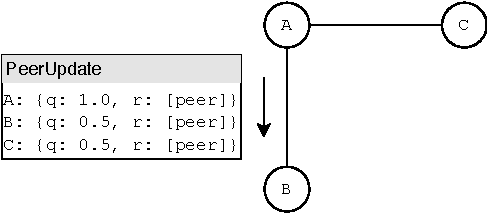
\includegraphics[width=0.45\textwidth]{graphics/design/peer-update-send.pdf}
\caption{Peer sends update containing its direct connections.}
\label{fig:peer-update-send}
\end{figure}

\begin{figure}
\centering
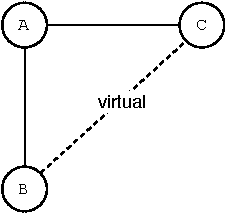
\includegraphics[width=0.45\textwidth]{graphics/design/peer-update-recv.pdf}
\caption{Peer received connection update and added a virtual connection.}
\label{fig:peer-update-recv}
\end{figure}
